\documentclass{article}

\usepackage[utf8]{inputenc}
\usepackage[T1]{fontenc}
\renewcommand*\familydefault{\sfdefault}
\usepackage[francais]{babel}
\usepackage{graphicx}
\usepackage{tabularx}
\usepackage{listings}
\usepackage[left=4cm, right=4cm]{geometry}

\title{\textbf{Répartiteur de charge}}
\author{%
  Clément \textsc{Delpech} \\
  Armel   \textsc{Mangean} \\
  Idrissa \textsc{Sokhona}
}%
\date{\today}

\begin{document}

  \maketitle
  \thispagestyle{empty}
  \newpage

  \tableofcontents
  \thispagestyle{empty}
  \newpage
 
  \setcounter{page}{1}

  \section{Analyse}
  \subsection{Définition du sujet}
    
    % Petite intro / Definition dans les très grandes lignes du sujet
    Une problématique récurrente dans le monde informatique est
    l'optimisation des ressources disponibles. Dans un réseau les
    ressources sont souvent inégalement utilisées. Une meilleure
    utilisation de ces ressources pourrait être obtenu en permettant à
    ces machines de s'échanger des tâches. C'est le but d'un système
    de répartition de charge.
        
    Afin de mieux comprendre ce qui est demandé voici quelques
    définitions des termes techniques employés.
    
    \paragraph{Tâche} Dans notre système une tâche l'execution d'un
      programme. On pourra considérer plus tard le degré
      d'interactivité que l'on souhaite gérer (gestion des E/S
      standards, gestion des fichiers, interface graphique...)
      
    %\paragraph{Un n\oe{}ud, un site} Une station de travail UNIX dans
    %  l'implémentation demandé

    \paragraph{Placement réparti} Ordonnancement de programmes i.e. choix
      d'un processeur pour un processus parmis un ensemble de
      machines. C'est une manière de tirer parti des ressources
      inutilisées.
      
    % Dynamique à détailler si on a le temps
    \paragraph{Placement dynamique et statique} Dans le cadre du
      placement statique avant le démarrage du système de répartion sera
      associé à une tâche un processeur. Cette tâche ne pourra
      qu'être executé sur ce processeur même si celui-ci est
      surchargé. Dans le cadre du placement dynamique le processeur où
      s'executera une tâche sera déterminé pendant l'execution.
              
    % TODO bonus - Eventulement accompagner d'un schéma comme celui du cours de Folliot
    \paragraph{Partage et équilibrage de charge} Il existe deux grandes
      stratégies de placement dynamique. La première stratégie est
      nommée partage de charge. Lorsque la charge globale d'une
      machine dépasse un seuil caractérisant la surcharge, il devient
      nécessaire de déplacer quelques unes de ces tâches. Le but du
      partage de charge est de maximiser le débit d'exécution moyen
      des tâches. La seconde stratégie de placement est nommée
      équilibrage de charge. À chaque instant le système de
      répartition essaye de conserver un équilibre dans la répartition
      de la charge globale. Pour cela il determine une charge idéale
      que chacune des machines tend à expérimenter. Cette charge
      idéale est la moyenne des charges individuelles du système.

    %\paragraph{Coopératif} Placement décidé grâce à la coopération
    %  de l'ensemble des machine.

    %\paragraph{Connaissance de l'état global} La coopération permet
    %  d'avoir une réprésentation de l'ensemble du système (cependant
    %  inexacte du au temps de transmissions de données).

    \paragraph{Centralisation} Si l'on considère une implémentation
      décentralisé de ce système alors chaque n\oe{}ud a les mêmes
      prérogatives. Chaqun doit connaitre l'état du système ce qui
      impose soit un échange important de message passant
      difficilement à l'échelle soit un système d'échange
      d'information entre les n\oe{}ud complexe (connaissance
      partielle de l'état du système sur un n\oe{}ud). De plus, cela
      implique une connaissance approximative de l'état du système.
      Une approche centralisé defini les n\oe{}uds comme esclave
      soumis à un n\oe{}ud spécifique coordinateur. Quand un n\oe{}ud
      souhaite transferer une tâche, il envoie une demande au
      coordinateur qui choisit alors un n\oe{}ud cible en utilisant
      l'ensemble des information à sa disposition. On parlera aussi
      d'approche maitre-esclave ou bien client-serveur.      
      
    \paragraph{}
    L'objectif de ce projet est d'aboutir à la mise en \oe{}uvre
    effective d'un ordonnancement de processus sur un ensemble des
    machine. C'est à dire, à un instant donnée, déterminer le
    placement d'une tâche sur la machine la plus capable de la traiter
    en fonction de la charge de chacune des machines du parc. Le
    programme consiste en une couche d'abstraction intermediaire entre
    le système d'exploitation et les programmes à executer.
        
    \begin{figure}[h!]
      \centering
      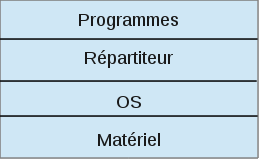
\includegraphics[width=0.58\textwidth]{img/couches_du_systeme.png}
      \caption{Couches d'abstrations présente dans un noeud}
    \end{figure}
    
  % Dans cette partie on doit définir toutes les problématiques associé
  % càd à quelles questions on devra répondre dans la partie conception
  \subsection{Compréhension des problèmes}
    
    La mise en place d'une telle solution pose un ensemble de
    questions auquelles il est nécessaire de répondre. Il est évoqué
    dans le sujet quatres grandes problématiques lié à la répartition.

    \begin{itemize}
      \item Evaluation de la charge de chaque machine
      \item Definition de la surcharge
      \item Choix de la tâche à déplacer 
      \item Choix des machines
    \end{itemize}

    Pour chacune de ces questions il est nécessaire de définir une
    politique définissant la manière dont on y répond. Aux politique
    répondant à ces questions s'ajoute une politique de tolérance aux fautes.

    \subsubsection{Politique d'information}

      Par définition, le système étant réparti il y a une dispersion
      des données importante. Le module d'information consiste à
      définir les informations devant être collectées, les instants
      pendant lesquels ces informations sont collectées, à partir de
      quels n\oe{}uds elles sont collectées.

      % A completer?
      \paragraph{Évaluation de la charge} Une bonne évaluation de la
        charge est cruciale pour notre appliction, l'efficacité et la
        réactivité de notre application en dépend. La charge de chaque
        machine constitue donc une information essentielle devant être
        recueillie. 

      % Mettre un schema?
      \paragraph{Répartition de l'information} Il existe deux méthodes
        de récolte d'information de la charge. La première est une
        politique où l'information est récoltée à la demande, ce qui
        permet de minimiser le nombre de messages échangés. Le
        principal inconvénient étant que l'information peut ne pas
        être suffisamment à jour dans le cas où les évenements qui
        lancent la récolte ne se produisent pas assez souvent. La
        seconde est une politique où l'information est récoltée
        périodiquement. Avec cette méthode la définition de la période
        est cruciale, trop grande on retrouvera le même inconvenient
        qu'avec une récolte évenementielle, trop petite les messages
        de contrôles risquent de saturer le réseau.
      
    \subsubsection{Politique de transfert}

      Le module de transfert est responsable de déterminer si un
      n\oe{}ud est dans un état approprié pour participer à un
      transfert de tâche comme source ou comme receveur.

      \paragraph{Évalutation de la surcharge} Afin de décider s'il est
        possible ou necessaire de faire un transfert il est possible
        de se référer à un seuil au delà du quel on considère être
        surchargé. Ce seuil peut être fixe ou bien dynamique,
        dépendant de l'activité du système de répartition.

      \paragraph{Décision de placement} Dans le cas du partage de
        charge, lors du dépassement de seuil de surcharge il est
        necessaire d'emetter une décision de placement pour chaque
        nouvelle tâche.  Dans le cas de l'équilibrage de charge un
        décision est requise à chaque nouvelle tâche sans contrainte
        de seuil.

    \subsubsection{Politique de localisation}

      Ce module est responsable de trouver les n\oe{}uds, émetteur et
      recepteur, étant les meilleures candidats au transfert d'une
      tâche. On répond donc ici au problème du choix de la machine
      réceptrice.

      \paragraph{Approche serveur} La première approche basée sur
        un modèle serveur consiste à permettre aux machines pouvant
        accueillir des tâches supplémentaires de proposer leurs
        services. Lorsqu'une machine estime pouvoir accueillir une
        tâche elle émet une offre de service. Les n\oe{}uds subissant
        une surcharge répondent en conséquence. La machine détermine
        alors le n\oe{}ud le plus approprié à ce transfert de tâche.

      \paragraph{Approche client} La seconde approche, à l'inverse,
        se base sur le modèle \textit{client} et consiste à permettre
        aux machines subissant une surcharge de demander les services
        d'une des autres machines du système. Lorsqu'une machine
        souhaite transferer une tâche elle emet une demande de partage
        de charge. Les n\oe{}uds aptes à offrir leur aide répondent en
        conséquence. La machine détermine alors le n\oe{}ud le plus
        approprié.
          
     %\paragraph{} Dans la pratique le choix d'un approche dépendra
     %   fortement si l'on est dans un système avec centralisation ou
            
    %\subsubsection{Politique de séléction}
    %  La politique de sélection est responsable du choix des tâches à
    %  transférer. Nous distinguons trois politiques principales de
    %  sélection.

    %  \begin{itemize}
    %    \item choisir une des tâches ayant contribué à ce que le nœud 
    %            devienne surchargé.
    %    \item choisir n'importe quel tâche c'est à dire toute les 
    %            tâches sont considérées comme éligibles.
    %    \item choisir une tâche approprié. Le choix d'une tâche 
    %           appropriée peut nécessiter une bonne connaissance sur la
    %            tâche aussi bien que sur les machines destinataire.
    %  \end{itemize}
        
    % NB on doit gerer une machine qui tombe, mais pas un remise en route auto
    \subsubsection{Politique de tolérance aux fautes}

      On doit gérer les pannes franches des machines, c'est-à-dire les
      machines ne répondant plus. D'une part on doit pouvoir détecter
      la panne ce qui implique d'interoger chaque machine à intervalle
      de temps réguilier. D'autre part, on doit faire en sorte que la
      panne ne pertube pas le bon déroulement de notre système. On
      pourra donc spécifier explicitement que les tâches interrompues
      ne se sont pas terminée correctement. Ainsi, la machine les
      ayant transféré pourra de nouveau les faire executer dans le
      système réparti.

\newpage
\section{Conception}

  Dans cette partie, nous allons nous intéresser aux données présentes
  sur chaque n\oe{}ud, aux messages envoyés entre sites et aux
  algorithmes de chacun des modules étudiés ci-dessus.

  \subsection{Topologie}

    Par soucis de simplicité et de faisabilité -- n'ayant jamais
    implémenté de système réparti -- nous organiserons notre système
    de placement selon un modèle maître-esclaves. En effet, la
    centralisation des données simplifie la réalisation d'un tel
    système. Le rôle d'un esclave est de participer au placement
    réparti nottamment en exécutant les tâches qui lui sont
    confiées. Il a connaissance de l'identité du maître ainsi que de
    sa propre charge. Le rôle du maître est de coordoner le placement
    réparti. Ainsi, le placement est réalisé en centralisant les
    données ainsi que la prise de décision. Le maître a connaissance
    de tous les esclaves ainsi que de la charge de chacun des
    esclaves. La machine maître endosse le double rôle de maître
    et d'esclave.
        
    \begin{figure}[h!]
      \centering
      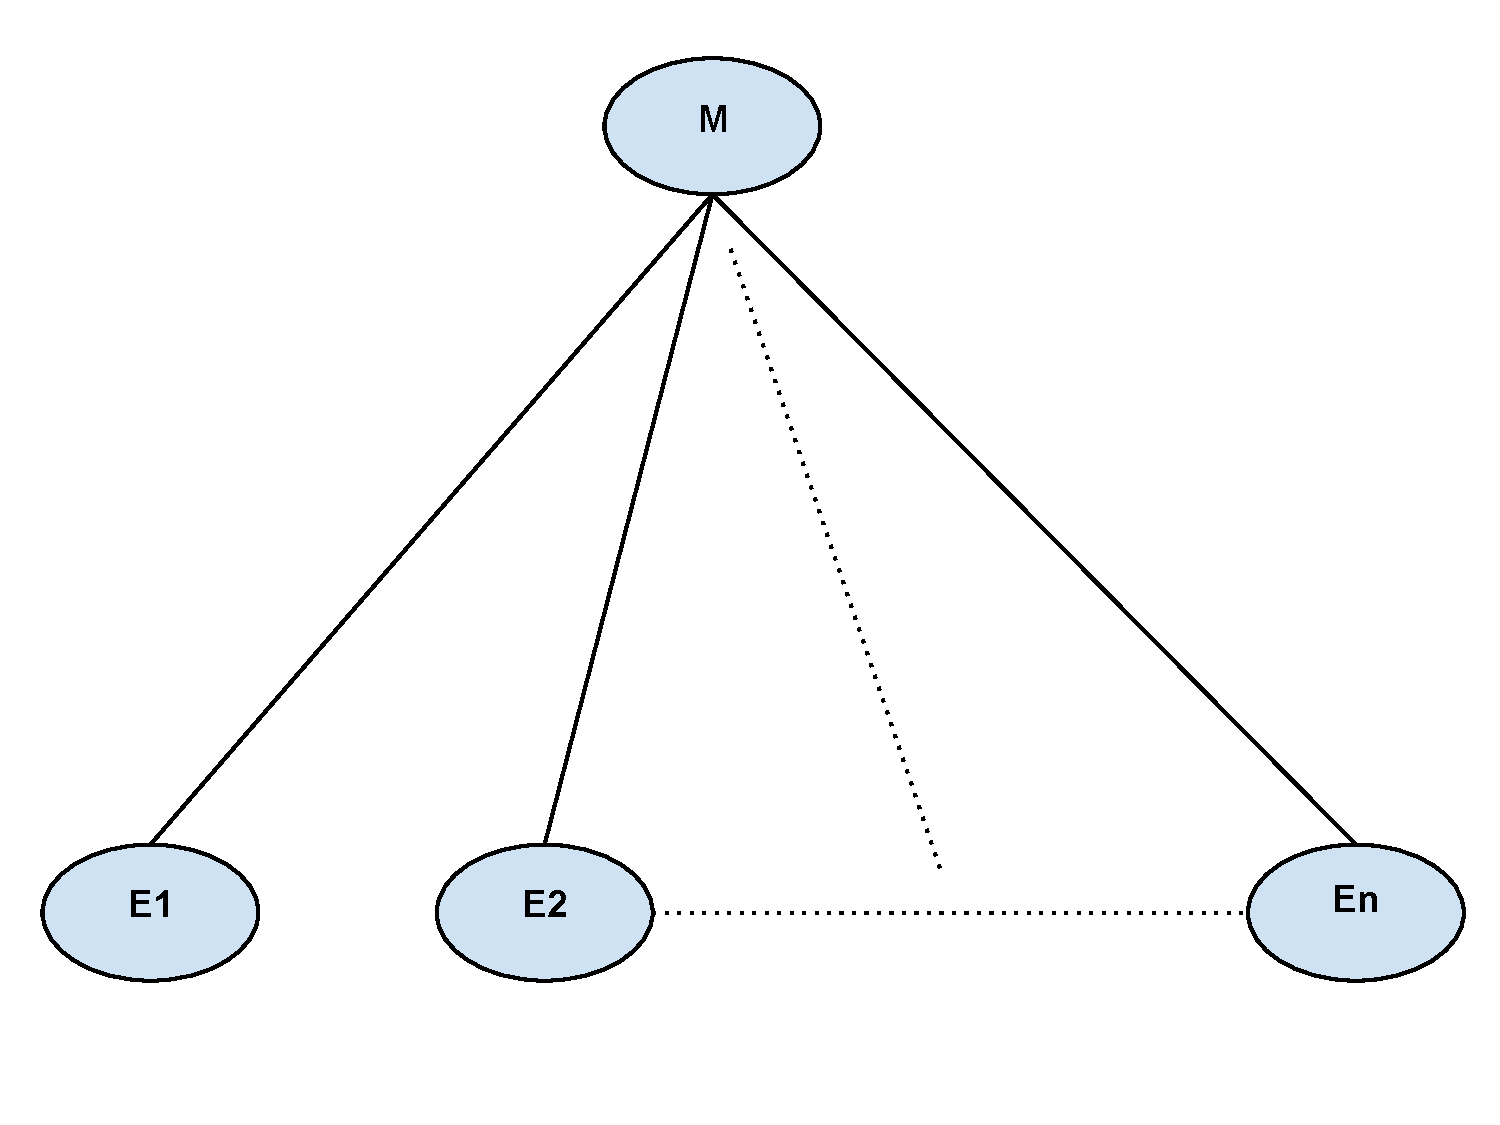
\includegraphics[scale=0.45]{img/topologie.pdf}
      \caption{Topologie du système de placement réparti}
    \end{figure}
      
    % petit argumentation sur les autre possibilité et les raison du
    % choix

    Notons que cette solution peut poser problème dans le cas d'une
    machine maitre peu performante ou d'un nombre d'esclave trop
    grand. Un système totalement décentralisé effacerai le problème de
    goulot d'étrangelement au niveau du maîtere. Compte-tenu des
    exigences de notre projet, on peut imaginer que le nombre de
    machines restera raisonnable (inférieure à 20), ainsi la gestion
    des esclaves par un ordinateur de bureau récent restera trés
    largement supportable.
        
  \subsection{Interface utilisateur}

    Concernant les interaction avec l'utilisateur nous avons choisi la
    voie de la simplicité. L'application se lancera via un terminal.
    A l'interieur de l'application l'interface sera en ligne de
    commande avec un nombre de commandes réduit. Chaque commande
    traitera une opération bien distincte.

    \begin{itemize}
      \item S'integer au système
      \item Executer une tache dans système réparti
      \item Quitter l'application
      \item Observer le système
    \end{itemize}
        
  \subsection{Calcul de la charge d'une machine}

    Il est capital de définir correctement ce que sera la charge dans
    notre application afin d'obtenir de bonnes performances. Une
    solution simple est de considérer le nombre de processus à l'état
    prêt, attendent le processeur. Il faudra considérer l'ensemble des
    processus c'est-à-dire aussi ceux s'executant en dehors du système
    de placement réparti. Afin de renforcer la validité d'utilisation
    de ce facteur on pourra le pondérer en fonction des particularités
    de chaque machine.
      
    \subsection{Module d'information}

      Ce module concerne la gestion de l'état ainsi que de la charge
      du système. Compte-tenu de la topologie choisie, les
      informations gobales seront centralisés au niveau du maître. Il
      devra gérer deux ensembles de données à savoir l'état des
      clients et la charge des client.
        
      Les donnés seront récupéré par interrogation (polling) des
      esclaves par le maître. Chaque esclave recalcule sa charge à
      chaque fois que le maitre lui enverra une requête. Le polling se
      fera dès lors que le système aura besoin de données à jour.

      %\begin{itemize}
      %  \item polling de tout les esclaves lorsque le maître cherche à
      %          placer une nouvelle tâche.
      %  \item polling de tout les esclaves lors de l'élection d'un 
      %          nouveau maître.
      %  \item polling de tout les esclaves lorsque l'utilisateur
      %          demande l'état du système.
      %  \item polling du nouvel arrivant lors de l'insertion d'une
      %          nouvelle machine
      %\end{itemize}

    \subsection{Module de transfert}

      Afin de minimiser les échanges entre les différents sites, on
      laisse la possibilité aux esclaves d'exécuter leurs propres
      tâches sans passer par le maître. le transfert de tâche sera
      uniquement effectué lorsque l'escalve se considérera surchargé.
      Dans ce cas de figure il demandera au maître une machine
      destinatrice sur laquelle il pourra envoyer la tâche.
        
      \paragraph{Cas partage} C'est la politique de placement que nous
        implémenterons dans un premier temps. Chaque esclave possede
        un seuil qui lui est propre. Au départ le seuil sera fixe.
      
      \paragraph{Cas équilibrage} Cette politique sera mise en place
        dans un second temps. Le seuil sera calculé par le maître
        comme une moyenne des charges des esclaves.

    \subsection{Module de localisation}

      La décision de placement se fera au niveau du maître.
      Lorsqu'une nouvelle tâche est crée sur un esclave surchargé,
      celui-ci demande au maître l'identité d'une machine sur laquelle
      il peut envoyer cette tâche. Le maître interroge l'ensemble des
      esclaves pour obtenir leur charges puis il répond au site
      demandeur avec l'identité de la machine la moins chargé. Cette
      machine peut tout à fait être l'esclave ayant fait la
      demande. Une fois cette identité obtenue, la machine cliente
      communique la tâche à la machine cliente.
      
    \subsection{Tolérance aux pannes}

      La détection de panne d'une machine est réaliser lors du
      dépassement du délais fixé par un temporisateur. Le maître
      réalisera cette détéction en s'appuyant sur les messages de
      récolte de la charge des esclaves. Une fois la panne détecté, il
      signalera aux autres esclaves qu'une machine a brusquement
      quitté le système afin que les tâches qui étaient placées sur
      cette machine puissent être relancées.
      
      Un esclave détectera la panne du maître lors d'une demande de
      placement de tâche. Cette détéction initiera une éléction d'un
      nouveau maître. Le noeud élu endossera le rôle du maître afin de
      permettre au système de reprendre de manière transparente.

    \subsection{Intégration et retrait de machines}

      L'intégration d'un nouveau n\oe{}ud au placement se réalise comme
      suit. La machine fait parvenir son identité et sa charge au
      maître. Une fois que le maître a connaissance de la nouvelle
      machine il met à jour l'état global et envoie une confirmation
      à la machine demandeuse.
      
      La retrait d'un n\oe{}ud du placement se déroule
      ainsi. Lorsqu'un utilisateur demande le retirait de sa machine
      du système de placement réparti celle ci annonce au maître
      qu'elle n'accepte plus de tâche. Dès lors que l'execution de
      toute les tâches qu'elle comprend se termine elle annonce au
      maître qu'elle se retire, le maître mets alors à jour l'état
      global. Dans le cas d'un arret brutale le fonctionnement connu
      par un esclave est celui décrit en cas de faute franche.

  % Part 2:
%  - Protocols
%  - Seeder/leecher
%  - Software
%  - eMule, Limewire, Bittorrent, Freenet, Kazaa, Napster
%  - Security
%  - Trackers
%  - P2P file sharing free : Skype
%  - CDN/DNS

% Sources
% howstuffWorks.com
% Cours NetArch de Fourmaux
% http://www.slideshare.net/uschmidt/peertopeer-systems
% http://en.wikipedia.org/wiki/Peer-to-peer

% 
\section{How it works?}

  \begin{frame}
    \tableofcontents[currentsection, hideothersubsections]
  \end{frame}

  \subsection{Technical challenges of P2P}
    \begin{frame}
      \frametitle{\secname}
      \framesubtitle{\subsecname}
      \begin{itemize}
        \item How Peers know each other?
        \item How to find the required file in the network?
        \item How to be sure all peers participate ?
        \item How to guarantee file availability? (seeding)
      \end{itemize}
    \end{frame}

  \subsection{Napster the grandpa}
    \begin{frame}
      \frametitle{\secname}
      \framesubtitle{\subsecname}
      \begin{itemize}
        \item Based on central index server 
        \item Server know all peers
        \item P2P only for file transfert
        \item Still some client/server !
        \item No mecasim to promote seeding
      \end{itemize}
      \begin{figure}
        \centering
        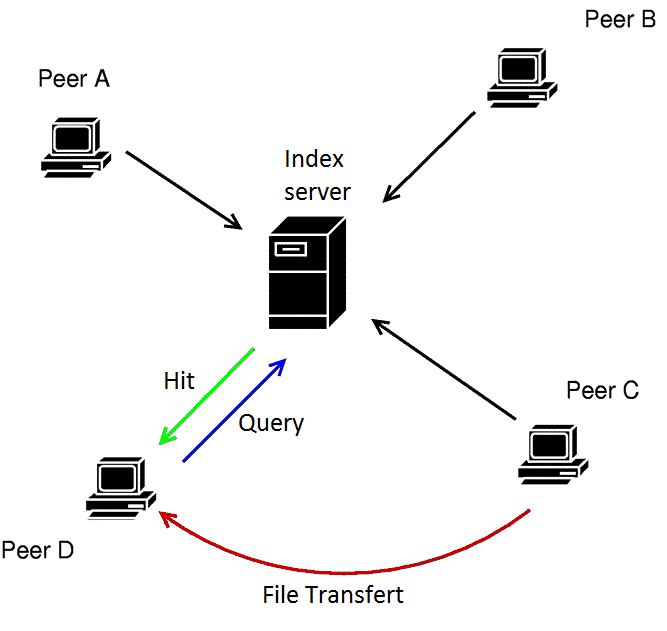
\includegraphics[scale=0.2]{img/P2-napsterProtocol2_colored.png}
        %\caption{Napster architecture}
      \end{figure}
    \end{frame}


  \subsection{Gnutella the unknown child}
    \begin{frame}
      \frametitle{\secname}
      \framesubtitle{\subsecname}
      \begin{itemize}
        \item Fully distibuted
        \item A peer know a few amount of his fellow
        \item Search by flooding
        \item Still no mechanism to promote seeding
      \end{itemize}
      \begin{figure}
        \centering
        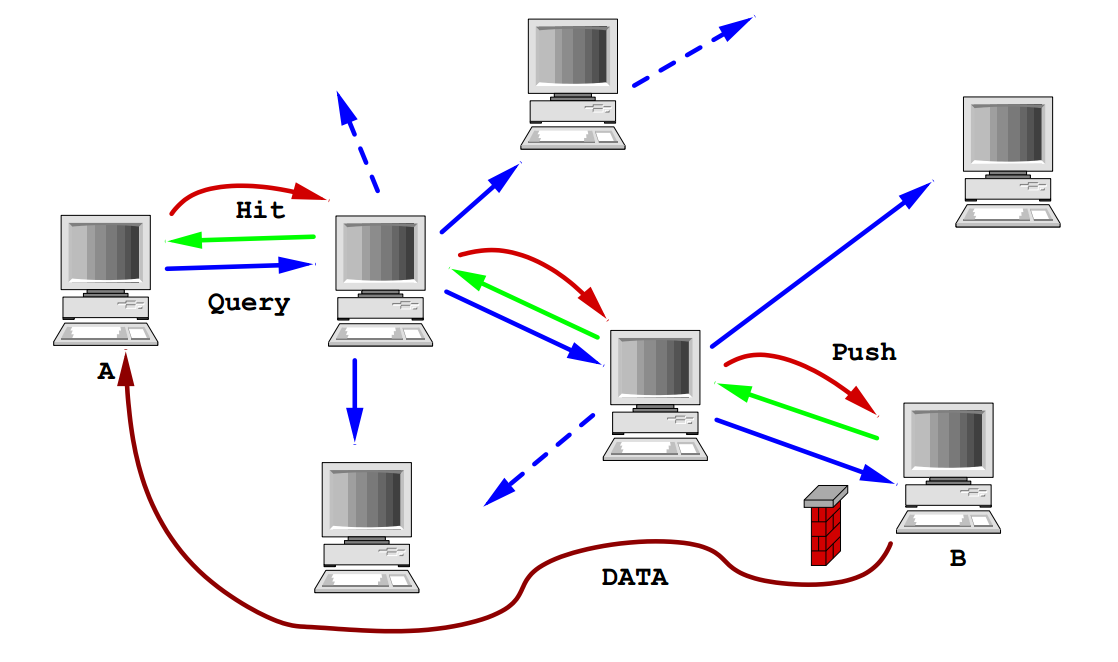
\includegraphics[scale=0.30]{img/P2-gnutellaProtocol.png}
      \end{figure}
    \end{frame}
    
    
  \subsection{Bittorent the long-living}
    \begin{frame}
      \frametitle{\secname}
      \framesubtitle{\subsecname}
      \begin{itemize}
        \item File search outsourced with .torent file
        \item A Tracker oversees the distribution
        \item Files are divided in chunk
        \item tit-for-tat policy
      \end{itemize}
    \end{frame}
   

  \subsection{Other P2P systems}
    \begin{frame}
      \frametitle{\secname}
      \framesubtitle{\subsecname}
      \begin{itemize}
        \item Internet routing
        \item IM, VoIP (SIP Protocol, Skype)
        \item CDN and others cloud based applications
        \item Grid computing, DNS
      \end{itemize}
    \end{frame}

   %% Le rapport final reprendra le rapport de conception (corrigé)
  % + mise en œuvre (réalisations) + manuels instal/utilisateur
  % + jeu de tests
  % + pblms rencontrés, etc.)

%%configuration de listings
\lstset{language=C} % TODO - configurer correctement la coloration de code

\section{Implémentation et mise en œuvre}
 
  \subsection{Choix de la technologie}
    \paragraph{}
     Pour la réalisation de notre projet, le choix nous a été donné entre 
     socket et RPC pour la communication entre machines. 
     Nous avons porté notre choix sur RPC grâce à différents  avantages 
     qu'il présente par rapport et à certains critères que nous avons définis. 

     \paragraph{}
     \noindent Facilité de programmation :
     RPC (appel de procédures à distance) cache la complexité des protocoles 
     de communication et permet la génération automatique de code (à l'aide
     de RPCGEN) pour le client et pour le serveur qui couvre la communication 
     (les talons ou souches). Les appels sont fait comme des appels de procédures
     en local (sauf qu'il ne permet pas le passage par adresse).
     
     \paragraph{}
     \noindent Portabilité et Héterogenéité :
     RPC utilise le standard XDR pour l'envoie de messages entre machines
     
 \subsection{Génération du code RPC}
    \paragraph{utilisation de rpcgen}
    Nous avons dans un premier temps procédé à la génération du code rpc
    en utilisant l'outil rpcgen. Dans le fichier \verb"PlacementReparti.x" nous
    avons défini les structures de données de notre programme (tel que
    vu dans la Figure 11). A cela nous avons spécifié dans l'interface
    les procédures qui seront appelés à distances  tel que présenté
    ci-dessous.
    
    
    \paragraph{}
    \noindent Procédures distantes pour une machine esclave :
    
    \begin{verbatim}
      unsigned long quiEstPlusGrand(unsigned long) = 1;
      unsigned long tuConnaisMaitre() = 2;
      string collecterDonneesMachine() = 3;
      void jeSuisInitialise() = 4;
      int recolterCharge() = 5;
      bool_t executerDistante(ProgrammeExporte) = 6;
      void terminerProgramme(RetourFinExecution) = 7;
    \end{verbatim}
    
    \paragraph{}
    \noindent Procédures distantes supplémentaire pour une machine maître :
    \begin{verbatim}
      string collecterDonneesMachines() = 1;
      bool_t enregistrerEsclave(MachineEsclave) = 2;
      unsigned long choisirMachineDistante() = 3;
    \end{verbatim}
    
    \paragraph{Organisation des fichiers}
    A partir des fichier générées par rpcgen nous avons réorganisé le code
    afin de le placer dans des fichier correspondant aux interfaces défini
    précédemment. Ainsi nous avons un fichier header par module (information,
    transfert, localisation et IHM), ainsi qu'un dernier fichier pour 
    gérer le démarrage de notre application (\verb"InitialiserPlacement.h").
    
    Nos fichiers sources sont organisés en trois parties. Une partie 
    contenant les procédures d'appel côté client (tel que généré par
    rpcgen), situé dans des fichiers nommés \verb"ModuleXXXAppel.c". Les deux
    autres parties sont situés dans les fichiers sources (\verb"ModuleXXX.c").
    Chaque ficher de module contient d'une part les procédures locales à
    une machine et d'autre part les procedures distantes (côté serveur).
    
    % TODO bonus - mettre un schéma d'arborescence
  
    
  \subsection{Integration d'une machine au placement}
    \paragraph{}
    Nous avons choisi dans un premier temps de nous intéresser à
    l'intégration d'une machine dans notre système afin de pouvoir
    travailler sur un base minimale de notre application et d'étendre au
    fur et à mesure les fonctionnalités. Le choix à été fait de rendre
    totalement transparent l'intégration d'une machine au système, pour
    cela nous avons utilisé la fonction broadcast de RPC. la procédure 
    \verb"InitialiserPlacementReparti" s'occupe de determiner par un premier
    broadcast si il existe déjà un maître actif sur le réseau. S'il n'y
    a pas de réponse, la procédure lance une élection afin d'élire un
    nouveau maître.
    Une fois le type de n\oe{}ud déterminé, la procédure ce charge
    d'enregistrer les fonctions qui pourront être appelées à distance.
    Il ne reste plus alors qu'à lancer le serveur RPC avec la fonction RPC
    \verb"svc_register" et d'attendre les requêtes des autres machines du placement 
    avec la fonction RPC \verb"svc_run". 
  
  \subsection{Interface (IHM)}
    \paragraph{}
    L'interface utilisateur que nous avons créée s'inspire très
    fortement de la commande \verb"ftp". Notre binaire se lance sans argument,
    une fois l'étape d'integration passée, notre programme laisse la 
    main à l'utilisateur où il pourra tapez une des 5 commandes de notre
    application (EXECUTE, QUIT, KILL, ADMIN ou HELP). Pour parser la
    commande nous avons utilisé les fonction de la librairie standard C
    \verb"fgets", \verb"strtok" et \verb"strcmp". 
    Étant donné que nous avons lancé le serveur RPC avant d'attendre les
    commandes de l'utilisateur, nous avons dû créer un nouveau thread.
    Ainsi la fonction \verb"entrerCommande", qui se charge de parser les 
    commandes et d'aiguiller vers les fonctions adéquats, est lancé dans
    un thread séparé.
  
  \subsection{Exécution d'un programme}
    \paragraph{}
    L'execution d'un programme (ou tâche) se fait par un appel des 
    fonctions \verb"fork" puis \verb"exec", en passant en parametre la ligne de
    commande donné par l'utilisateur. Chaque machine possède deux liste
    de tâche : une liste des tâches propres à la machines, qu'elles 
    soient éxecutées localment ou exportés sur une machine distante ; et
    une liste des tâches importées. On aura, associé à ces deux listes, 
    deux compteur pour le nombre d'entrées qui faciliteront la gestion.
    
    \subsubsection{Exécution locale}
    
      \paragraph{}    
      Un des principal problème à résoudre a été la détection de la
      terminaison d'un programme. Étant donné que la fonction \verb"wait" est
      bloquante nous ne pouvons pas l'executer dans le même thread que
      notre programme principal. Nous avons donc décidé de créer un
      thread pour chaque tâche éxecuté localement qui se chargera de 
      traiter la fin du processus fils. 
      
      Une autre solution envisagé était de redéfinir le signal
      SIGCHLD mais celle-ci n'était pas satisfaisante car il est
      impossible d'attendre le processus de pid voulu.

      
      % TODO mettre l'image sur github 
      \begin{figure}[h!]
        \centering
        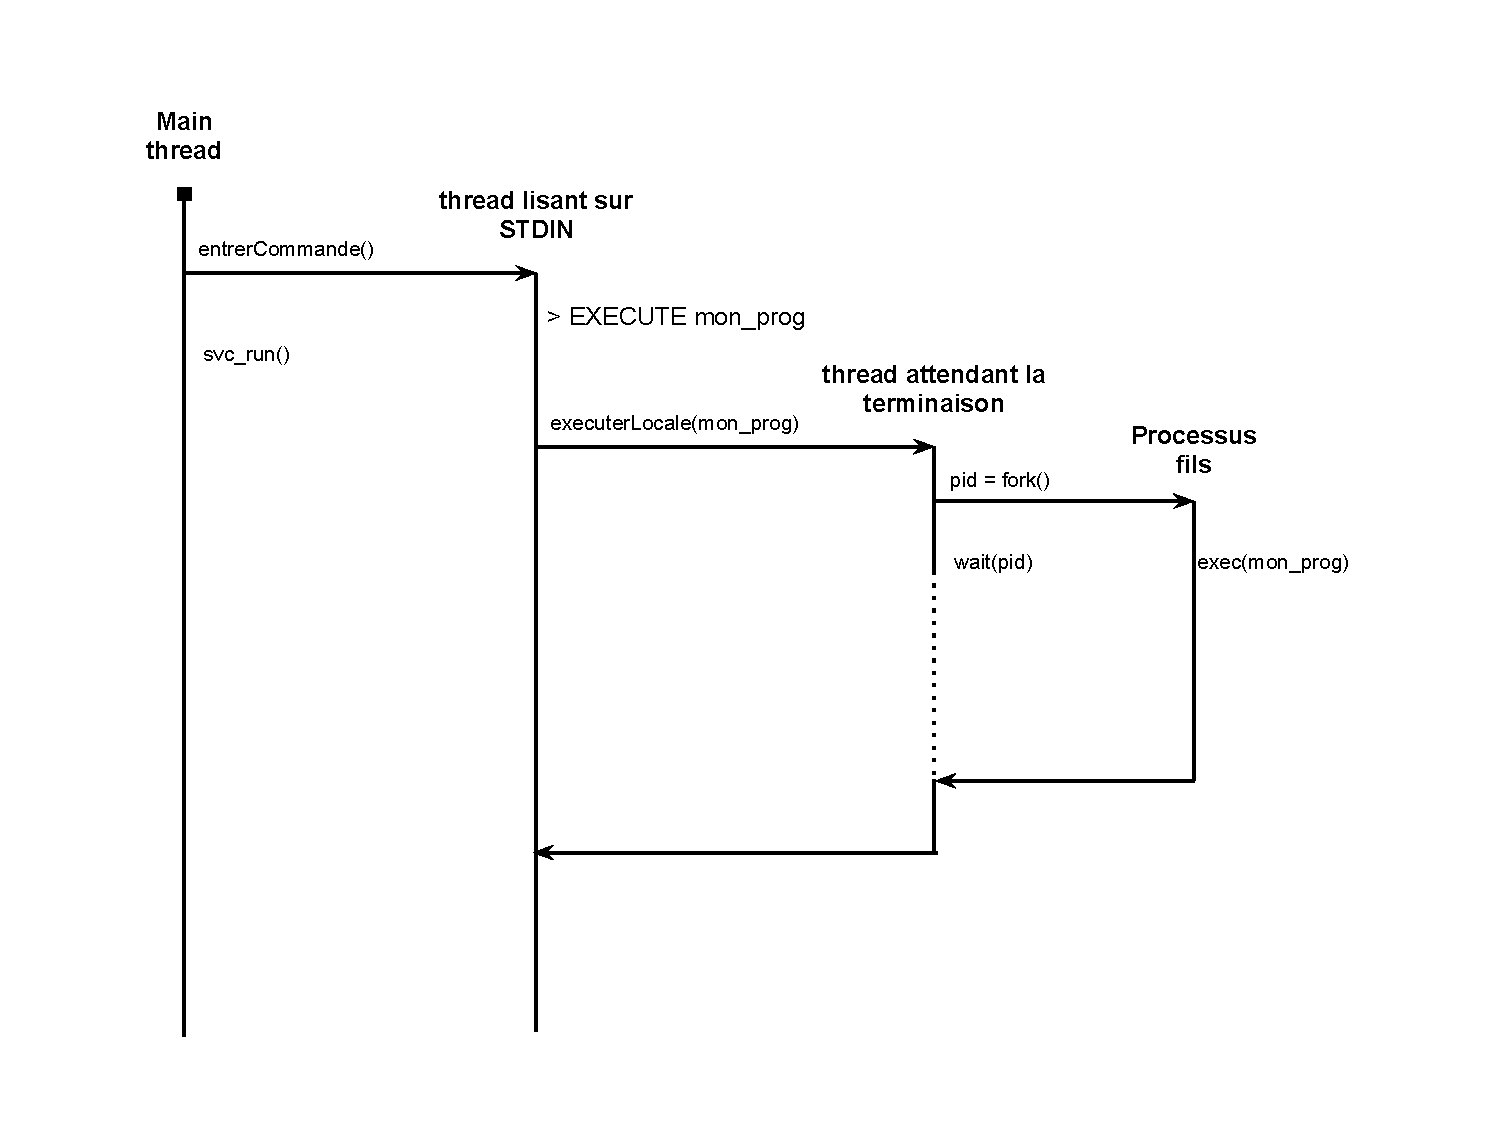
\includegraphics[scale=0.6]{img/execution_locale.pdf}
        \caption{Threads et processus impliqués dans l'éxecution d'un 
                 programme sur une machine locale}
      \end{figure}
    
  \subsubsection{Exécution à distance}
    \paragraph{}
    L'exécution à distance se fait par appel de la fonction 
    \verb"executerDistance" qui se charge de transmettre les informations
    nécessaire à l'éxecution du programme. De la même manière que lors
    de l'exécution locale, la machine (distante) exécutant le programme 
    créera un thread d'attente qui se chargera de notifier la machine 
    appelante. Du fait de ce choix, la notification de terminaison est 
    asyncrone : la machine choisie pour l'éxecution se chargera de 
    notifier la fin du programme par l'appel de la procédure distante 
    \verb"terminerProgramme".
    
    
    
    
    
    % TODO - Redirection E/S : pas implementé
    % L'execution étant à distance, les entrées/sorties sont rédirigés 
    % afin que les affichages se fassent sur la machine appelante.
    
    \newpage
    
    % TODO mettre l'image sur github
    \begin{figure}[h!]
      \centering
      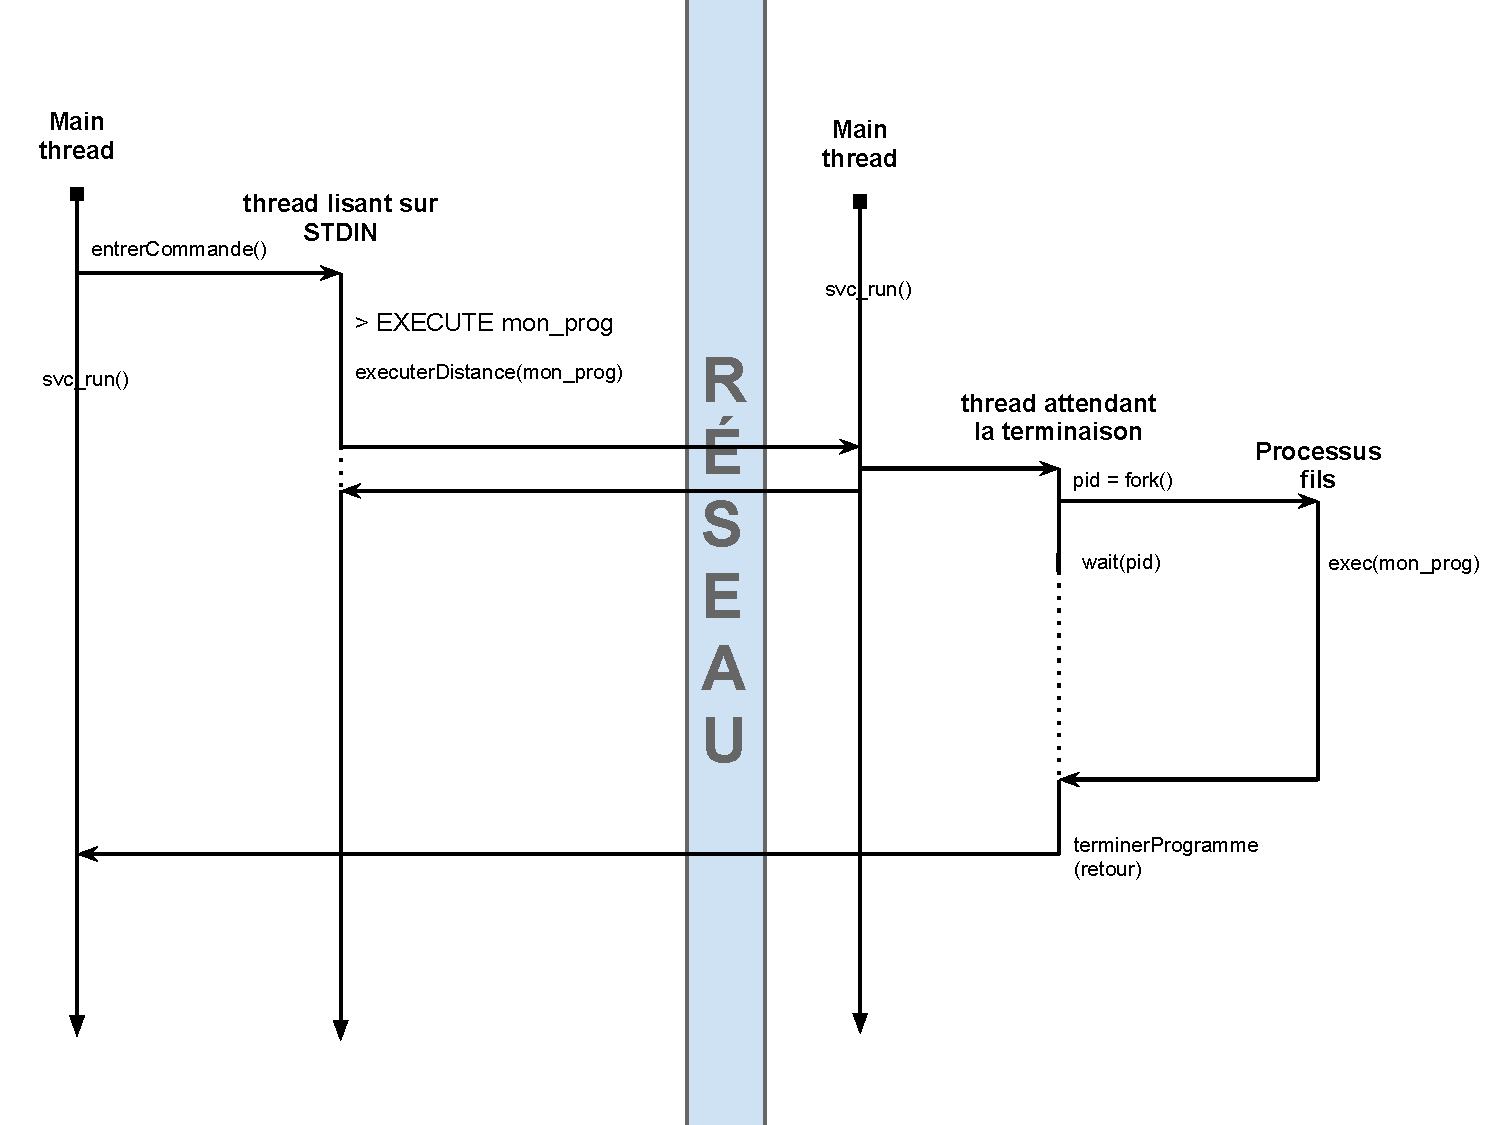
\includegraphics[scale=0.6]{img/execution_distante.pdf}
      \caption{Threads et processus impliqués dans l'éxecution d'un 
               programme sur une machine distante}
    \end{figure}

  \subsection{Calcul de la charge}
    \paragraph{}
    Étant donné que nous n'avons pas d'accès sur les informations des 
    processus au niveau noyau, nous avons utilisé les informations 
    disponibes en lecture dans le dossier \verb"/proc". A partir de ces 
    informations, nous avons établit la définition suivante :
    la charge correspont au nombre de processus utilisateur existant sur 
    la machine. Nous n'avons pas pris en compte la puissance du 
    processeur, notre environnement de test (salle de l'ARI) étant 
    constitué de machines de même puissance. La fonction de calcul pourra 
    tout de même être redefine afin de prendre en compte cette 
    problématique.
  
  \subsection{Choix de la machine}
    \paragraph{} 
    Nous avons implémenté 2 modes de  répartition : partage ou 
    équilibrage. Le choix du mode est fait "en dur" au moment de la 
    compilation mais il a été pris en compte la possibilité d'évolution 
    vers un choix au lancement du système, voir un changement pendant 
    l'execution du programme.
    
    \paragraph{Partage} 
    Dans le cas Partage, la décision se fait en partie localment. Si la 
    charge est inférieure au seuil, l'éxecution est locale, sinon on 
    demande au maître l'identité d'une machine pouvant exécuter la tâche
    à répartir. Le maître récoltera alors les charges des esclaves à 
    l'aide d'un broadcast de la procédure RPC \verb"recolterCharge", 
    puis choisira la première machine qui possède une charge inférieure 
    au seuil.
    
    \paragraph{Équilibrage}
    Dans le cas équilibrage, on interogerra systématiquement le maître 
    pour obtenir l'identité de la machine la plus apte.
    Lorsque le maître est interrogé il effectue un récolte de toutes les 
    charges de la même manière que pour le partage. Une fois la table 
    des charges à jour, le maître prend ça décision. Il choisira 
    systématiquement la machine la moins chargé.
    
  \subsection{Consultation de l'état de machines}
    % La consultation se fait par la commande ADMIN.
    Nous avons implémenté deux possibilité consultation : consultation 
    de l'état de toutes les machines (globale) et consultation de l'état
    d'une seule machine (locale).
    
    \paragraph{Consultation locale}
    La consultation locale correspont à un appel de la procédure distante 
    \verb"collecterDonneesMachine" sur la machine spécifié par 
    l'utilisateur (à l'aide de la commande ADMIN). Cette procédure se 
    charge de créer une chaine de caratères formaté pour l'affichage à
    partir des données locales (état, programmes exportés et programmes
    importés). La machine appelante se contente alors d'afficher la 
    chaine obtenue.
    % TODO
    % Voici un exemple d'affichage obtenu :
     
    
    \paragraph{Consultation globale}
    La consultation globale se fait par l'appel d'une procédure à 
    distance sur le maître pour obtenir l'état de l'ensemble des 
    machines du placement. Le maître effectue alors un collecte locale 
    sur l'ensemble des machines du système, puis agrège les chaînes 
    obtenu afin d'obtenir un texte prêt à être affiché.
    
    % TODO - pas codé
    %\paragraph{}
    %Afin de pouvoir observer le comportement du sysème, nous avons dans 
    %un seconde temps rendu l'affichage dynamique avec un fréquance de 
    %rafraichissement de 1 seconce. Pour cela nous avons utilisé la 
    %fonction alarm et redefini le signal SIGALRM (à l'aide de 
    %\verb"sigaction") sont utilisés pour raffraîchir l'affichage en
    %faisant une réexecution de la procedure à interval de temps régulier.
    
    
    \subsection{Retrait d'une machine}
    Comme vu précédemment, nous avons implémenté deux façon de quitter 
    le système. 
    
    \paragraph{}
    La première (commande \verb"KILL") n'attend pas la terminaison des 
    tâche mais notifie tout de même le maître de l'arrêt de la machine.
    Lors d'un arrêt ce ce type, la machine signal au maître sa 
    terminaison puis termine toutes les tâches en cours sur elle-même.
    Le maître notifira toutes les autres machines du placement afin 
    qu'elles gèrent elles-même la terminaison des tâches de la machine 
    venant de quitter.
    
    \paragraph{}
    La seconde (commande \verb"QUIT") attends la terminaison de toutes 
    les tâches, celles en cours sur la machine même mais aussi celles qu'elle 
    aura exporté sur d'autres machines. Pour cela la machine signalera 
    dans un premier temps au maître qu'elle n'accepte plus de tâche. 
    A chaque terminaison de tâche on testera nos compteurs afin de 
    savoir si le programme peut s'arrêter.
    
    % TODO
    \subsection{Gestions des pannes}
    
\section{Test}   
  \subsection{Environnement de test}
  
\section{Manuel d'utilisation}
   \subsection{Paramétrage et Compilation}
    \paragraph{}
    Le dossier de l'application présente les sous dossiers de notre code
    source : src (les xxx.c), include (les xxx.h) et bin (le fichier
    PlacementReparti). Dans le répertoire il y a un fichier Makefile qui
    permet la compilation et un fichier README.txt qui constitue notre
    manuel d'utilisation.

    \paragraph{}
    Par défaut, le type de répartition considéré est partage de charge,
    donc si on voudrait utiliser plutôt l'équilibrage de charge, il faut
    modifier les sources. Pour celà, il faut modifier dans le code
    source du fichier ModuleTransfert.c, situé dans le sous dossier src,
    la ligne typeRepartion = PARTAGE par typeRepartiton = EQUILIBRAGE.

    \paragraph{}
    Pour créer un éxecutable du programme, il faut ouvrir un terminal et 
    de se déplacer dans le dossier de l'application et, ensuite, 
    d'entrer la commande "make -f Makefile". L'exécutable est créé et se 
    situe dans le sous dossier bin.
    
    \subsection{Démarrage du placement}
    \paragraph{}
     Pour démarrer le placement, il faut se deplacer dans le sous 
     dossier bin du dossier du programme et d'entrer la commande
     "./PlacementReparti". Un message d'attente d'intégration ou une 
     invite d'entrée de commande ">" s'affiche. Dans le cas du message 
     d'attente, il faut patienter que l'invite soit affiché.
     
     \paragraph{}
     A l'aide de la commande HELP, on a la possibilité de connaitre tous 
     les commandes du placement  que voici : EXECUTE, QUIT, KILL, 
     ADMIN ou HELP. 
     \begin{verbatim}
       > HELP
     \end{verbatim}
     
     
    \subsection{Exécution d'un programme}
      \paragraph{}
      On exécute un programme avec la commande EXECUTE en lui fournissant 
      en paramètre le nom du programme et ses paramètre :
      \begin{verbatim}
        > EXECUTE /programme param1 param2 ...
      \end{verbatim}
      
      \paragraph{}
      La fin de l'exécution du programme est signalée.
      
       
      \subsection{Retrait d'une machine}
      \paragraph{}
      La commande QUIT entrée, la machine attend terminaison des 
      programmes exécutés sur elle des autres machines et, à la fin, elle 
      signale le retrait de la machine du placement.
      \begin{verbatim}
        > QUIT
      \end{verbatim}     
      
      \paragraph{}
      La commande KILL quant à elle met fin immédiatement les programmes 
      et retire la machine du placement
      \begin{verbatim}
        > KILL
      \end{verbatim}
      
      
    \subsection{Consulter l'état des machines}
      \paragraph{}
      La commande ADMIN nous permet de consulter l'état d'une machine ou 
      de l'ensemble de machines du placement. 
      
      \paragraph{}
      D'une machine, il faut entrer la commande avec un paramètre 
      l'adresse de la machine :
      \begin{verbatim}
        > ADMIN 192.168.1.4
      \end{verbatim}      
      
      \paragraph{}
      De toutes les machines, il faut entrer la commande avec le 
      paramètre étoile ou sans :
      \begin{verbatim}
        > ADMIN *
        
        > ADMIN
      \end{verbatim}
      


\end{document}

%% Exigences du rapport 
 %% Le Rapport de conception doit contenir :
  % - Définition du sujet
  % - Compréhension des problèmes
  % - Présentation des choix effectués
  % - Interface utilisateur
  % - Découpage en module
  % - Architecture globale du système (spécification des interfaces
  %   entre modules, spécification des différents messages échangés
  %   entre les processus répartis).
  % La solution doit être modulaire (i.e. composée de modules regroupant
  % des entités de même nature) et extensible (i.e. devant permettre
  % l'intégration de fonctionnalités supplémentaires.
  %
 %% Le rapport final reprendra le rapport de conception (corrigé)
  % + mise en œuvre (réalisations) + manuels instal/utilisateur
  % + jeu de tests
  % + pblms rencontrés, etc.)

%% Nota Bene :
 %  - Bien distinguer la partie qui developpe sur les politiques À
 %    DERTERMINER et celle qui parle des modules définissant des
 %    méthodes concrètes de réalisation.
 %  - Pas de politique de seléction pour le placement réparti
 %    dynamique dans la thèse de B. Folliot.
 %  - Le calcul de la charge ne se fait pas en fonction de
 %    l'utilisation CPU parce que le multitasking ça existe !
